\mode<presentation>
{
  \usetheme{Boadilla}
}

%\usepackage[english]{babel}
\usepackage[utf8]{inputenc}

% Note: using version 2.0-alpha3
\usepackage[cache]{minted}
\setminted{frame=single}

% Hour-long talk

\title{Type-Directed TDD in Rust}
\subtitle{A case study using FizzBuzz}
\author{Franklin Chen \\ \url{http://franklinchen.com/}}
\date[\href{http://www.meetup.com/Pittsburgh-Code-Supply/events/183483622/}{Pittsburgh Code and Supply}]{July 21, 2014 \\ \href{http://www.meetup.com/Pittsburgh-Code-Supply/events/183483622/}{Pittsburgh Code and Supply}}

\subject{Talks}

\AtBeginSection[]
{
  \begin{frame}<beamer>{Outline}
    \tableofcontents[currentsection,subsectionstyle=hide]
  \end{frame}
}

\begin{document}

\maketitle

\begin{abstract}
  An expressive static type system is one of the most joyful and
  powerful tools for prototyping, designing, and maintaining
  programs. In this performance-theatrical presentation, I will
  provide a taste of how to use types, in conjunction with tests, to
  drive iterative development of a particular program, the famous
  FizzBuzz problem. We will solve generalizations of this problem,
  changing and adding requirements, to illustrate the pleasures and
  benefits of ``type thinking''.

  The Rust language will be used as the vehicle for this
  demonstration, but the techniques apply immediately to any
  industrial-strength statically typed language, such as Scala, Haskell,
  OCaml, F\#, and Swift.

  (Note: this presentation will use live human volunteers to play the
  roles of various programming concepts.)
\end{abstract}

\begin{frame}
  \titlepage
\end{frame}

\section*{Outline}

\begin{frame}{Outline}
  \tableofcontents[subsectionstyle=hide]
\end{frame}

% Since this a solution template for a generic talk, very little can
% be said about how it should be structured. However, the talk length
% of between 15min and 45min and the theme suggest that you stick to
% the following rules:  

% - Exactly two or three sections (other than the summary).
% - At *most* three subsections per section.
% - Talk about 30s to 2min per frame. So there should be between about
%   15 and 30 frames, all told.

\section{Introduction}

\subsection{Goals}

\begin{frame}{Goals of this presentation}
  \begin{itemize}
  \item Give a taste of a \alert{practical} software development \alert{process} that is:
    \begin{itemize}
    \item \alert{test}-driven
    \item \alert{type}-directed
    \end{itemize}
  \item Show everything for real (using Rust):
    \begin{itemize}
    \item project build process
    \item testing frameworks
    \item all the code
    \end{itemize}
  \item Use \texttt{FizzBuzz} because:
    \begin{itemize}
    \item problem: easy to understand
    \item modifications: easy to understand
    \item fun!
    \end{itemize}
  \item Encourage you to explore a modern typed language; now is the time!
    \begin{itemize}
    \item Recently, Apple ditched Objective C for its new language \href{https://developer.apple.com/swift/}{Swift}!
      
\includegraphics[height=0.75cm]{swift-hero.png}
    \end{itemize}
  \end{itemize}
\end{frame}

\subsection{Test-driven development (TDD)}

\begin{frame}{Test-driven development (TDD)}
  \begin{itemize}
  \item Think.
  \item Write a test that \textcolor{red}{fails}.
  \item Write code until test \textcolor{green}{succeeds}.
  \item Repeat, and \textcolor{green}{refactor} as needed.
  \end{itemize}

  \begin{block}{\href{http://martinfowler.com/articles/is-tdd-dead/}{Is TDD dead?}}
    Short answer: No.
  \end{block}
\end{frame}

\subsection{Type systems}

\begin{frame}{Type systems}
  \begin{block}{What is a type system?}
    A \alert{syntactic} method to \alert{prove} that bad things can't happen.
  \end{block}

  \begin{block}{``Debating'' types ``versus'' tests?}
    \begin{itemize}
    \item Let's use both types and tests!
    \item But: use a \alert{good} type system, not a bad one.
    \end{itemize}
  \end{block}

  \begin{block}{Some decent practical typed languages}
    \begin{itemize}
    \item \href{http://ocaml.org/}{OCaml}: 20 years old
    \item \href{http://www.haskell.org/}{Haskell}: 20 years old
    \item \href{http://www.scala-lang.org/}{Scala}: 10 years old
    \item \href{http://developer.apple.com/swift/}{Swift}: $<2$ months old
    \item \href{http://www.rust-lang.org/}{Rust} (still not at 1.0!)
    \end{itemize}
  \end{block}
\end{frame}

\begin{frame}<article|handout>{Poor versus decent type systems}
  \begin{block}{Poor type systems}
    \begin{itemize}
      \mode<article|handout>{
        \item (Developed using 1960s-1970s knowledge)
      }
    \item C, C++, Objective C
    \item Java
    \end{itemize}
  \end{block}

  \begin{block}{Decent type systems}
    \begin{itemize}
      \mode<article|handout>{
        \item (Developed using 1980s-1990s knowledge)
      }
    \item ML (\href{http://www.smlnj.org/}{Standard ML}, \href{http://swift.org/}{OCaml}, \href{http://fsharp.org/}{F\#}): I first used for work in 1995
    \item \href{http://www.haskell.org/}{Haskell}: I first used for work in 1995
    \item \href{http://www.scala-lang.org/}{Scala}: first released in 2004
    \item \href{http://developer.apple.com/swift/}{Swift}: announced by Apple on June 2, 2014!
    \item \href{http://www.rust-lang.org/}{Rust}: not yet version 1.0
    \end{itemize}
  \end{block}
\end{frame}

\section{Original FizzBuzz problem}

\subsection{Original FizzBuzz problem}

\begin{frame}{Original FizzBuzz problem}
  \begin{block}{FizzBuzz defined}
    Write a program that prints the numbers from 1 to 100.

    But for multiples of three, print ``Fizz'' instead of the number.

    And for the multiples of five, print ``Buzz''.

    For numbers which are multiples of both three and five, print ``FizzBuzz''.
  \end{block}
\end{frame}

\subsection{Starter code: main driver}

\begin{frame}[fragile]{Starter code: main driver}
  \begin{block}{
\includegraphics[height=0.75cm]{rust-logo-128x128-blk-v2.png}}
    Rust: a modern systems programming language for efficiency and safety in time, space, and concurrency.
  \end{block}

  \inputminted{rust}{Main1.rs}

  \begin{itemize}
  \item Type-directed design: separate out effects (such as printing to terminal) from the real work.
  \item Type-directed feedback: compilation fails when something is not implemented yet.
  \end{itemize}
\end{frame}

\subsection{Compiling and testing with Cargo}

\begin{frame}[fragile]{Compiling and testing with Cargo}
  \begin{block}{
\includegraphics[height=0.75cm]{Cargo-Logo-Small.png}}
    \href{http://crates.io/}{Cargo}: build tool for Rust
  \end{block}

  \begin{block}{Features}
    \begin{itemize}
    \item Library dependency tracking.
    \item \mintinline{console}{cargo build}
    \item \mintinline{console}{cargo test}
    \end{itemize}
  \end{block}

  \begin{block}{My wish list, based on Scala \href{http://www.scala-sbt.org/}{SBT}}
    \begin{itemize}
    \item Triggered compilation and testing
    \item Interactive REPL
    \end{itemize}
  \end{block}
\end{frame}

\begin{frame}[fragile]{First compilation failure}
  \texttt{src/main.rs}:
  \inputminted{console}{testQuick.console}
\end{frame}

\begin{frame}[fragile]{Write type-directed stub}
  \inputminted{rust}{Main2.rs}

  \begin{block}{Write wanted type signature}
    \mintinline{rust}{fail!} is convenient for stubbing.
    \begin{itemize}
    \item In Rust standard library
    \item Causes whole task to fail
    \end{itemize}
  \end{block}
\end{frame}

\subsection{Write acceptance test (simplified)}

\begin{frame}[fragile]{Write acceptance test (simplified)}
  \inputminted[gobble=2]{rust}{MainSpec1.rs}

  \mode<article>{
    A realistic acceptance test would involve handling I/O, but an elegant
    technique for modularizing that is outside the scope of this presentation.
  }
\end{frame}

\begin{frame}<article|handout>[fragile]{TDD in Swift}
  \inputminted{swift}{MainSpec1.swift}
\end{frame}

\begin{frame}[fragile]{Test passes type check, but fails}
  \inputminted{console}{testQuick2.console}
\end{frame}

\begin{frame}[fragile]{Outside-in: for a \mintinline{rust}{fizzbuzz} module}
  Types are shapes to assemble logically.

  \inputminted{rust}{Main4.rs}

  \begin{itemize}
  \item \mintinline{rust}{range(include, exclude)} returns an \alert{iterator}.
  \item \mintinline{rust}{map} takes an iterator of one type to an iterator of another:
  \begin{center}
    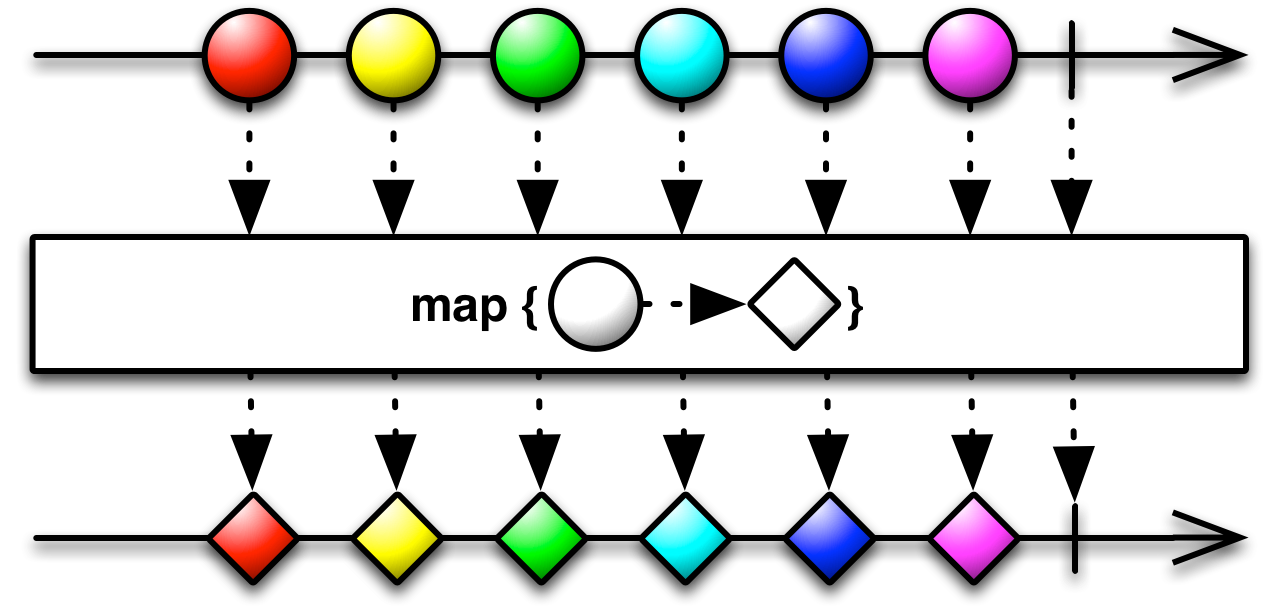
\includegraphics[height=2.5cm]{map.png}
  \end{center}
  \item Therefore: need to implement function \mintinline{rust}{fizzbuzz::evaluate: int -> String}.
  \end{itemize}
\end{frame}

\begin{frame}<article|handout>[fragile]{Swift version of driver}
  \inputminted{swift}{Main4.swift}
\end{frame}

\subsection{Test-driven units}

\begin{frame}[fragile]{Implement new \mintinline{rust}{fizzbuzz} module}
  A failing acceptance test drives \alert{discovery} of
  \begin{itemize}
  \item A \alert{unit}, \mintinline{rust}{fizzbuzz}
  \item A function with a particular type,
    \mintinline{rust}{int -> String}
  \end{itemize}

  \inputminted{rust}{FizzBuzz1.rs}

  \begin{block}{\alert{Types} are better than \alert{comments} as \alert{documentation}!}
    Comments are not checkable, unlike types and tests.
  \end{block}
\end{frame}

\begin{frame}[fragile]{First part of \alert{unit test}: example-based}
  Manually write some \alert{examples}.

  \inputminted[gobble=2]{rust}{FizzBuzzSpec1.rs}
\end{frame}

\subsection{Property-based tests}

\begin{frame}[fragile]{The joy of property-based tests}
  \href{https://github.com/BurntSushi/quickcheck/}{QuickCheck for Rust}: a framework for writing \alert{property-based} tests.

  \inputminted[gobble=2]{rust}{FizzBuzzSpec2.rs}

  \begin{block}{Winning features}
    \begin{itemize}
    \item Auto-generates \alert{random} tests for each property (100 by default).
    \item \alert{Type-driven}: here, generates random \mintinline{rust}{int} values.
    \end{itemize}
  \end{block}
\end{frame}

\begin{frame}<article|handout>{Property-based testing for Swift?}
  I hope someone writes a property-based testing framework for Swift!
\end{frame}

\begin{frame}[fragile]{Property-based tests (continued)}
  \inputminted[gobble=2]{rust}{FizzBuzzSpec3.rs}
\end{frame}

\subsection{Solving the FizzBuzz problem}

\begin{frame}[fragile]{A buggy and ugly solution}
  \inputminted[gobble=2]{rust}{FizzBuzzIf.rs}

  \inputminted{console}{testQuick3.console}
\end{frame}

\begin{frame}{Booleans are evil!}
\begin{block}{\href{http://en.wikiquote.org/wiki/Colossal\_Cave\_Adventure}{Maze of twisty little conditionals, all different}}
  \begin{center}
    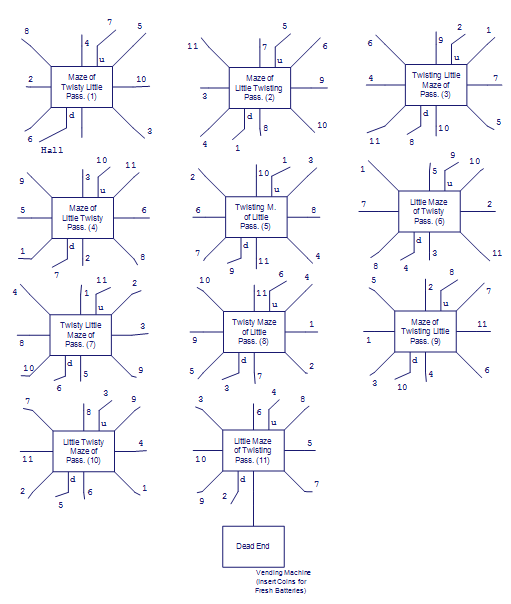
\includegraphics[height=3cm]{dmaze.png}
  \end{center}

  \begin{itemize}
  \item Too easy to write incorrect sequences of nested, combined conditionals.
  \item \href{http://existentialtype.wordpress.com/2011/03/15/boolean-blindness/}{Overuse of Booleans} is a type \alert{smell}.
  \end{itemize}
  \end{block}
\end{frame}

\begin{frame}<article|handout>{Why booleans are evil}
  \begin{block}{No help from type system}
    \begin{itemize}
    \item Conditions can be arbitrary: depend on \alert{any} combination of data.
    \item Multiple conditions: combinatorial explosion (two conditions led to four cases).
    \item Possibly overlapping conditions: order dependency subtleties.
    \item Possibly duplicated checking of the some condition.
    \end{itemize}
  \end{block}
\end{frame}

\begin{frame}[fragile]{Pattern matching organizes information}
  \inputminted{rust}{FizzBuzz2.rs}

  \begin{block}{Winning features}
    \begin{itemize}
    \item Visual \alert{beauty} and clarity.
    \item No duplicated conditionals.
    \item No ordering dependency.
    \item \alert{Type checker} verifies \alert{full coverage} of cases.
    \end{itemize}
  \end{block}
\end{frame}

\begin{frame}[fragile]{Example of non-exhaustive pattern matching}
  \inputminted{rust}{FizzBuzz2Bad.rs}

  \inputminted{console}{testQuick4.console}
\end{frame}

\begin{frame}<article|handout>[fragile]{Swift digression: pattern matching}
  The same solution, in Swift:

  \inputminted{swift}{FizzBuzz2.swift}
\end{frame}

\begin{frame}[fragile]{Acceptance test passes}

  \inputminted{console}{testQuick5.console}

  \begin{block}{Done?}
    No. Client wants more features.
  \end{block}
\end{frame}

\section{FizzBuzz 2: user configuration}

\subsection{Adding new features}

\begin{frame}{Adding new features}
  \begin{block}{Client wants to:}
    \begin{itemize}
    \item Choose two \alert{arbitrary} divisors in place of \mintinline{rust}{3} and \mintinline{rust}{5}
      \begin{itemize}
      \item such as \mintinline{rust}{4} and \mintinline{rust}{7}
      \end{itemize}
    \item Choose other \alert{arbitrary} words in place of \mintinline{rust}{"Fizz"} and \mintinline{rust}{"Buzz"}
      \begin{itemize}
      \item such as \mintinline{rust}{"Moo"} and \mintinline{rust}{"Quack"}

      \end{itemize}
    \end{itemize}
  \end{block}
\end{frame}

\subsection{Type-driven refactoring}

\begin{frame}{Type-driven refactoring}
  \begin{block}{Types mean: refactoring is much more fun!}
  \begin{itemize}
  \item Add \alert{new} tests.
  \item Change types and code: to make new tests \alert{type check}.
  \item \alert{Refactor} original code and tests: use new APIs.
  \item Keep passing the \alert{old} tests.
  \item Delay writing code for new features.
  \end{itemize}
  \end{block}
\end{frame}

\begin{frame}[fragile]{More features means more types}
  Change \mintinline{rust}{fizzbuzz::evaluate} to \mintinline{rust}{defaults::fizzbuzzer}:
  \inputminted{rust}{Main5.rs}

  Add new types to \mintinline{rust}{FizzBuzz} module:
  \inputminted{rust}{FizzBuzz3.rs}
\end{frame}

\begin{frame}[fragile]{New default configuration}
  \inputminted{rust}{Defaults1.rs}
\end{frame}

\begin{frame}[fragile]{More types means more tests}
  Write new property-based test over \alert{arbitrary} user configurations:
  \inputminted[gobble=2]{rust}{FizzBuzzSpec6.rs}
\end{frame}

\subsection{Refining types}

\begin{frame}[fragile]{Problem: coarse \mintinline{rust}{Config} type}
  \inputminted{console}{testQuick6.console}

  \begin{itemize}
  \item \mintinline{rust}{0} as a divisor \alert{crashes}!
  \item We discovered client's \alert{underspecification}.
  \item Client says: meant to allow only divisors within \mintinline{rust}{2} and \mintinline{rust}{100}.
  \end{itemize}

  We need to:
  \begin{itemize}
  \item Add runtime \alert{validation} when \alert{constructing} \mintinline{rust}{Config}.
  \item Refine \mintinline{rust}{Config} random generator.
  \end{itemize}
\end{frame}

\subsection{Validation}

\begin{frame}[fragile]{Add (runtime) validation}
  \alert{Runtime} precondition contract: Rust's \mintinline{rust}{assert!} (very primitive; fails a task on failure):

  \inputminted{rust}{FizzBuzz3Validate.rs}
\end{frame}

\begin{frame}{A note on error handling}
  \begin{itemize}
  \item \alert{Rust does not have exceptions}!
    \begin{itemize}
    \item \href{http://blog.jessitron.com/2013/06/whats-dirtier-than-comments-exceptions.html}{Exceptions are evil} because they escape the type system.
    \end{itemize}
  \item Rust task failures are brutal.
  \item Outside scope of this presentation: principled type-based error handling using \href{http://doc.rust-lang.org/std/result/}{\mintinline{rust}{Result<T, E>}}: 
  \end{itemize}
\end{frame}

\begin{frame}<article|handout>[fragile]{Data validation can be critical!}
  \begin{block}{Digression: two ways to prevent \href{http://heartbleed.com/}{Heartbleed}}
    \begin{itemize}
    \item Instead of C: use a \href{http://en.wikipedia.org/wiki/Dependent_type}{dependently typed} safe systems language such as \href{http://www.ats-lang.org/}{ATS} for \href{http://bluishcoder.co.nz/2014/04/11/preventing-heartbleed-bugs-with-safe-languages.html}{compile-time TDD}.
    \item Even with C: use \href{http://martinfowler.com/articles/testing-culture.html}{good validation and testing practices}.
      \begin{itemize}
      \item A weaker type system is not an \alert{excuse} to skip
        write tedious validation code or tests!
      \end{itemize}
    \end{itemize}
  \end{block}
\end{frame}

\begin{frame}[fragile]{Improve \mintinline{rust}{Config} random generator}
  \inputminted[gobble=2]{rust}{FizzBuzzSpec7.rs}
\end{frame}

\begin{frame}[fragile]{New test runs further, stills fails}
  Refactor old code to \mintinline{rust}{fizzbuzz::evaluate}, to pass old tests and new test.

  \inputminted{rust}{FizzBuzz3Compile.rs}
\end{frame}

\section{FizzBuzz 3: \texttt{FizzBuzzPop} and beyond}

\subsection{Generalize to more than two divisors}

\begin{frame}[fragile]{Generalizing to more than two divisors}
  \begin{block}{Client wants \texttt{FizzBuzzPop}!}
  \begin{itemize}
  \item Given three divisors (such as 3, 5, 7).
  \item Given three words (such as \mintinline{rust}{"Fizz"}, \mintinline{rust}{"Buzz"}, \mintinline{rust}{"Pop"}).
    \mode<article|handout>{
  \item Create evaluator that given an integer prints:
    \begin{itemize}
    \item either a string combining a subset of the three words, or
    \item a numerical string if the integer is not a multiple of any of the three divisors
    \end{itemize}
    }
  \item Example: \mintinline{rust}{21} should output \mintinline{rust}{"FizzPop"}.
  \end{itemize}
  \end{block}
\end{frame}

\begin{frame}<article|handout>{Thought-driven development}
    Software development is not primarily about \alert{coding}, but \alert{thinking}.

  \begin{itemize}
  \item Deep fact: solving a more general problem is often easier than solving the specific problem.
  \item There are four important numbers in the Universe:
    \begin{description}
    \item[0] emptiness
    \item[1] existence
    \item[2] other (relationship)
    \item[many] community
    \end{description}
  \end{itemize}
\end{frame}

\subsection{More features means more tests and types (again)}

\begin{frame}[fragile]{More features means more tests}
  Write new tests for new \mintinline{rust}{defaults::fizzbuzzpopper}:

  \inputminted[gobble=2]{rust}{FizzBuzzSpec5.rs}

  Change configuration: to \mintinline{rust}{Seq} of pairs, instead of just two:
  \inputminted{rust}{Defaults2.rs}
\end{frame}

\begin{frame}[fragile]{More tests means more (or changed) types}
  \inputminted{console}{testQuick8.console}

  Change \alert{type} \mintinline{rust}{Config} to allow a sequence of pairs:

  \inputminted{rust}{FizzBuzz3Seq.rs}

  \mode<article|handout>{
    Note how our iterative development process promotes \alert{reuse} (here, of validation logic).
  }
\end{frame}

\begin{frame}[fragile]{Fix remaining type errors}
  Refactoring reveals need to implement case of more than two divisors.

  \inputminted{rust}{FizzBuzz3SeqCompile.rs}
\end{frame}

\begin{frame}<article|handout>{General observations}
  \begin{itemize}
  \item Return a sum of a subset of the configured words, if there is any divisor match.
  \item If there is \alert{no} divisor match, return the numerical string.
  \end{itemize}
\end{frame}

\begin{frame}[fragile]{More computation means more types}
  Associate each divisor with a ``rule'' that awaits input.

  \inputminted{rust}{FizzBuzz4.rs}

  \begin{block}{\texttt{FizzBuzz} demo time!}
    \begin{itemize}
    \item Two volunteers: each to play role of \mintinline{rust}{Rule}.
    \item One ``manager'' to combine two sub-results.
    \end{itemize}
  \end{block}
\end{frame}

\subsection{Demo}

\begin{frame}<article|handout>{Demo explanation}
  \begin{itemize}
  \item Given a sequence of rules and an integer: apply all the rules to the integer, then combine the partial results.
  \end{itemize}

\end{frame}

\begin{frame}[label=first-general,fragile]{Assemble the types}
  \inputminted{rust}{FizzBuzz5.rs}
\end{frame}

\begin{frame}[fragile]{A note on \mintinline{rust}{fold}}
  For any value of type \mintinline{rust}{Iterator<A>}, we can apply \mintinline{rust}{fold: (B, |B, A| -> B) -> B}.
  \begin{center}
    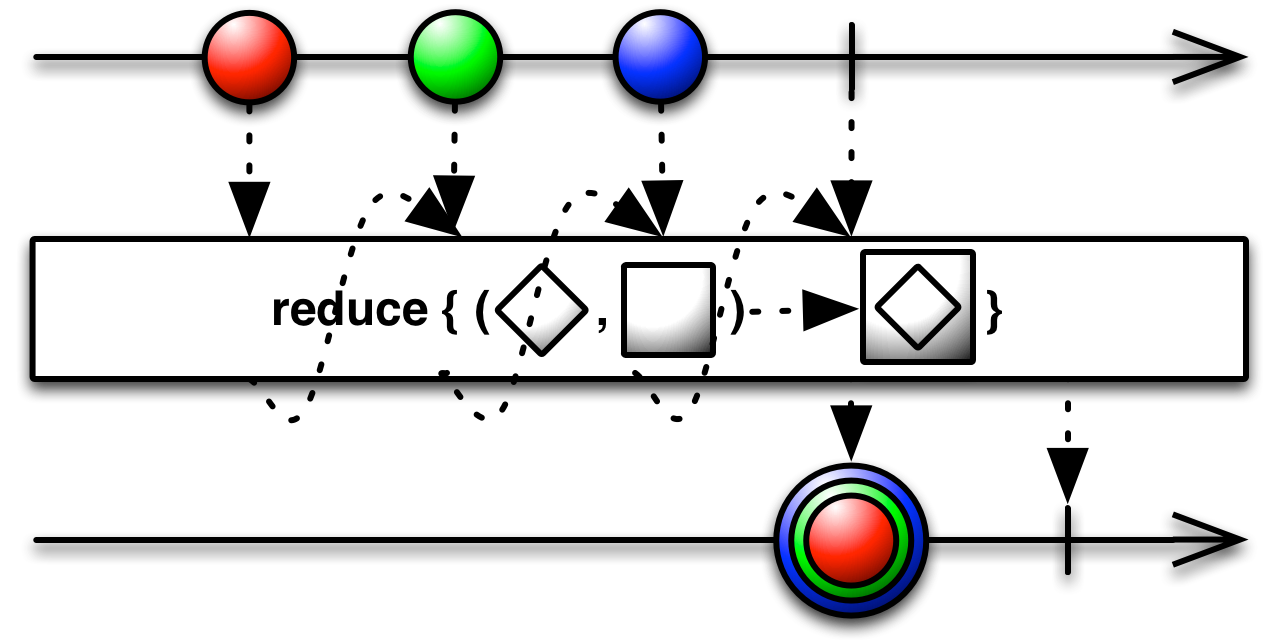
\includegraphics[height=2.5cm]{reduce.png}
  \end{center}

  Example: for \mintinline{rust}{Vec<String>}, fold with string concatenation \mintinline{rust}{+} returns the concatenation of all the strings in the vector.
\end{frame}

% Complicated, need to explain properly.
\begin{frame}[fragile]{Test failure: coarse types again}
  \inputminted{console}{testQuick9.console}

  \begin{block}{Demo time!}
    \begin{itemize}
    \item Configuration: \mintinline{rust}{vec![(3, ""), (5, "Buzz")]}
    \item Input: \mintinline{rust}{9} (note: divisible by \mintinline{rust}{2})
    \item Output: should be \mintinline{rust}{""} (because of the part divisible by \mintinline{rust}{3})
    \item Output was: \mintinline{rust}{"9"}
    \end{itemize}
  \end{block}
\end{frame}

\againframe<beamer>{first-general}

\begin{frame}[fragile]{Property-based testing rescued us again!}
  \begin{block}{Be honest: would you have caught this bug manually?}
    \begin{itemize}
    \item I didn't.
    \item I never wrote \texttt{FizzBuzzPop} examples testing empty strings.
    \item Property-based testing reveals \alert{unexpected} corner cases.
      \begin{itemize}
      \item (Empty ``fizz'' and ``buzz'' word strings).
      \end{itemize}
    \end{itemize}
  \end{block}
\end{frame}

\subsection{\mintinline{rust}{Option<A>} type}

\begin{frame}{An empty string is \alert{not} equivalent to no string}
  \begin{block}{Presence of something ``empty'' is \alert{not} equivalent to no thing.}
    Sending someone an empty email versus not sending any email.
  \end{block}
  
  Many programming languages get this wrong.
\end{frame}

\begin{frame}[fragile]{\mintinline{rust}{Option<A>} type}

  \mintinline{rust}{Option<A>} is one of two possibilities:
  \begin{itemize}
  \item \mintinline{rust}{None}
  \item \mintinline{rust}{Some(a)} wraps a value \mintinline{rust}{a} of type \mintinline{rust}{A}.
  \end{itemize}

  For example, \mintinline{rust}{Some(String::empty())} is not the same as \mintinline{rust}{None}.

  \inputminted{rust}{OptionExample1.rs}
\end{frame}

\begin{frame}[fragile]{Cleaning up the types}
  \inputminted{rust}{FizzBuzz6.rs}

  Useful type errors:

  \inputminted{console}{testQuick10.console}
\end{frame}

\begin{frame}[fragile]{Fix the type errors: our rule builder}
  \inputminted{rust}{FizzBuzz7Rule.rs}

  \begin{block}{Demo time!}
    \begin{itemize}
    \item (Instructions: for result \mintinline{rust}{Some(s)}, hold up the string, else don't hold up anything)
    \item Configuration: \mintinline{rust}{vec![(3, ""), (5, "Buzz")]}
    \item Input: \mintinline{rust}{9}
    \item Output: now correctly is \mintinline{rust}{""}
    \end{itemize}
  \end{block}
\end{frame}

\begin{frame}[fragile]{Fix the type errors: our evaluator}
  \inputminted{rust}{FizzBuzz7.rs}

  \begin{itemize}
  \item We need to write: \mintinline{rust}{addOption}
  \item Rust standard library provides: \mintinline{rust}{unwrap_or_else}
  \end{itemize}
\end{frame}

\begin{frame}[fragile]{``Addition'' for \mintinline{rust}{Option[String]}}
  \inputminted{rust}{FizzBuzz8.rs}
\end{frame}

\begin{frame}[fragile]{Getting \mintinline{rust}{A} back out of \mintinline{rust}{Option<A>}}
  \begin{block}{Do not lose information!}
    \mintinline{rust}{unwrap_or_else} inspects the \mintinline{Option<A>} value and either
    \begin{itemize}
    \item returns the value \mintinline{rust}{v} inside a \mintinline{rust}{Some(v)},
    \item or else returns the value from a closure.
    \end{itemize}
  \end{block}
\end{frame}

\begin{frame}<article|handout>[fragile]{Swift has two option types}
  Swift calls them ``optionals''.

  \begin{block}{Normal optional type}
    \begin{itemize}
    \item \mintinline{swift}{A?} is a type for each type \mintinline{rust}{A}.
    \item Must unwrap explicitly.
    \end{itemize}
  \end{block}

  \begin{block}{Implicit unwrapped optional type}
    \begin{itemize}
    \item \mintinline{swift}{A!} is a type for each type \mintinline{rust}{A}.
    \item Unfortunate type hole:
      \begin{quote}
        If you try to access an implicitly unwrapped optional when it
        does not contain a value, you will trigger a runtime error.
      \end{quote}
    \end{itemize}
  \end{block}
\end{frame}

\begin{frame}<article|handout>[fragile]{The same thing, in Swift}
  \inputminted{swift}{FizzBuzz8.swift}
\end{frame}

\subsection{Transform information; don't destroy it}

\begin{frame}[fragile]{Transform information; don't destroy it}
  Our complete code only uses \mintinline{rust}{if} in one place.

  \begin{block}{Bug cause: destroying information, using \mintinline{rust}{if}} 
    \begin{itemize}
    \item \mintinline{rust}{if i % n == 0 { word } else { String::new() }}
    \item \mintinline{rust}{if combined.is_empty() {i.to_string()} else {combined}}
    \end{itemize}
  \end{block}

  \begin{block}{Transforming information}
    \begin{itemize}
    \item To \mintinline{rust}{Option[String]}: \mintinline{rust}{if i % n == 0 { Some((*word).clone()) } else { None }}
    \item Back to \mintinline{rust}{String}: \mintinline{rust}{combined.unwrap_or_else(|| i.to_string())}
    \end{itemize}
  \end{block}

  \begin{block}{Type-directed design tip}
    We could have saved trouble \alert{up front}, by using precise \alert{types}.
    \begin{itemize}
    \item Avoid \mintinline{rust}{if}, when possible.
    \item Avoid \mintinline{rust}{String} (but required at I/O boundaries of program).
    \end{itemize}
  \end{block}
\end{frame}

\section{Parallel \texttt{FizzBuzz}}

\begin{frame}[fragile]{Parallelism}
  Some easy parallelism possible (not yet in Rust standard libraries):
  \begin{itemize}
  \item Use of \alert{map}.
  \item Use of \alert{fold}: parallelizable because of the monoid property:
  \begin{block}{\mintinline{rust}{Option<String>} is a \href{http://en.wikipedia.org/wiki/Monoid}{Monoid}}
  \begin{itemize}
  \item There is an identity element (\mintinline{rust}{None}).
  \item There is a binary associative operator (\mintinline{rust}{add_option}).
  \item \href{http://www.michael-noll.com/blog/2013/12/02/twitter-algebird-monoid-monad-for-large-scala-data-analytics/}{Fantastically important in practice!}
  \end{itemize}
  \end{block}
  \end{itemize}
\end{frame}

\begin{frame}[fragile]{Final (hypothetical) parallelized code}
  \inputminted{rust}{FizzBuzz9.rs}

  \begin{block}{Coding style tip}
    This level of conciseness is not always best: maybe too ``clever''?
  \end{block}
\end{frame}

\begin{frame}[fragile]{Final demo!}
  \begin{block}{Demo time!}
    \begin{itemize}
    \item Configuration: \mintinline{rust}{vec![(3, "Fizz"), (5, "Buzz"), (7, "Pop"), (2, "Boom")]}
    \item Tree of volunteers to simulate concurrency:
      \begin{itemize}
      \item Four at leaves.
      \item Two ``middle managers'' each handling two leaves.
      \item One top-level manager handling two middle managers.
      \end{itemize}
    \item Input: \mintinline{rust}{42}
    \item Output: \mintinline{rust}{"FizzPopBoom"}
    \end{itemize}
  \end{block}
\end{frame}

\begin{frame}{Parallelism summary}
  We discovered a theoretical speedup for generalized \texttt{FizzBuzz}:
  \begin{itemize}
  \item Sequential: $O(n)$
  \item Parallel: $O(\log n)$ (given $\log n$ processors, and omitting some technical subtleties)
  \end{itemize}

  Also, driver outer loop can be sped up:
  \begin{itemize}
  \item Sequential loop on 1 to $m$: $O(m)$
  \item Parallel loop: $O(1)$ (given $m$ processors)
  \end{itemize}
\end{frame}

\begin{frame}{Current (July 2014) Rust limitations}
  \begin{itemize}
    \item Rust \alert{closures}: still limited (work in progress!!).
    \item Scala/Swift/Haskell/etc. have unrestricted closures: less complex types, easy staged \alert{compilation}.
    \item Needs standard libraries for parallelism, using concurrency primitives such as \mintinline{rust}{spawn}.
    \item Need faster compiler, build system.
    \item Need better test frameworks.
  \end{itemize}
\end{frame}

\begin{frame}<article|handout>[fragile]{Bonus: the final code in Swift}
  \inputminted{swift}{FizzBuzzFinal.swift}
\end{frame}

\begin{frame}<article|handout>{Future work}
  \begin{itemize}
  \item Asynchronous
  \item Real-time
  \item Interactive
  \end{itemize}
\end{frame}

\section{Conclusion}

\begin{frame}{Conclusion}
  \begin{itemize}
  \item \alert{Tests} are great.
  \item \alert{Types} are great.
  \item Tests and types work hand in hand, driving design and program evolution.
  \item Modern typed languages such as Rust promote fun, correct programming!
  \item It's a great time to be learning and using a modern typed language.
  \end{itemize}

  \begin{block}{Code, slides, article}
    \begin{itemize}
    \item \url{https://github.com/franklinchen/type-directed-tdd-rust}
    \item The \href{https://github.com/FranklinChen/type-directed-tdd-rust/blob/master/presentation/article.pdf}{article} has more detail omitted in the presentation.
    \item The hyperlinks in all provided PDFs are clickable.
    \item Scala: \url{https://github.com/franklinchen/talk-on-type-directed-tdd-using-fizzbuzz}
    \item Swift: \url{https://github.com/franklinchen/fizzbuzz-swift}
    \end{itemize}
  \end{block}
\end{frame}

\appendix

\section*{\appendixname}

\begin{frame}<article|handout>{Some free online courses on modern typed functional programming}
  \begin{itemize}
  \item Using Scala: \href{http://www.coursera.org/course/progfun}{Functional Programming Principles in Scala} on Coursera, taught by Martin Odersky (inventor of Scala)
  \item Using Haskell: \href{http://www.edx.org/course/delftx/delftx-fp101x-introduction-functional-2126}{Introduction to Functional Programming} on EdX, taught by Erik Meijer (Haskell hero)
  \end{itemize}
\end{frame}

\end{document}

%%% Local Variables: 
%%% mode: latex
%%% TeX-master: "presentation"
%%% End: 
